\chapter{Introduction}

%Explain the context of your essay topic, so that the
%topic itself appears motivated, natural and important.bhvvnvn v vn  nv/KVKV
%
%\begin{figure}[h]
%\psfrag{A}{$d^2$}
%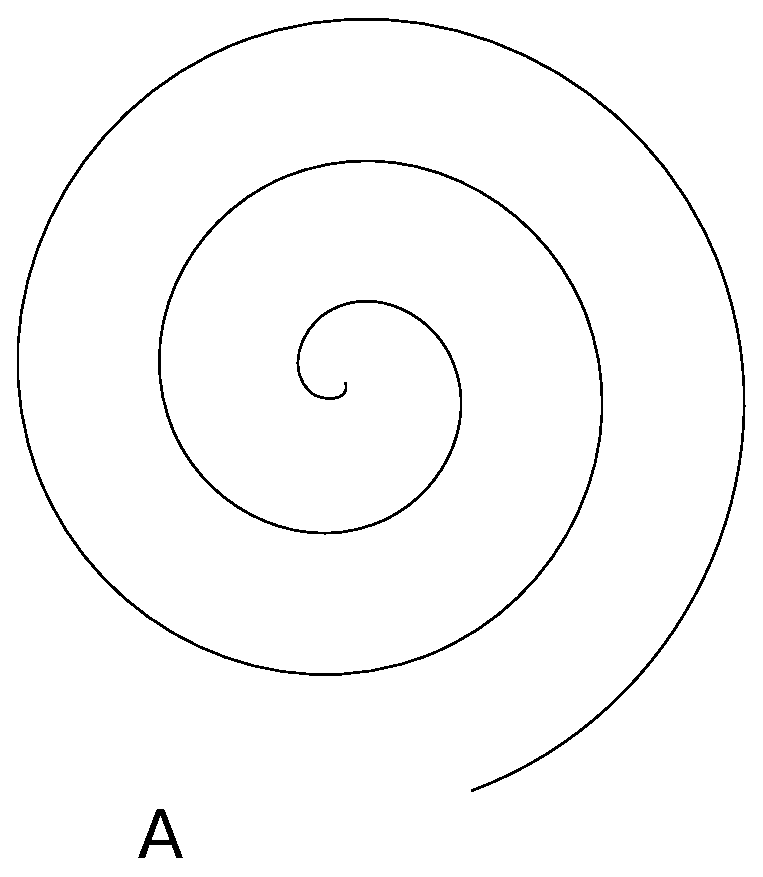
\includegraphics[scale=0.5]{images/drawing.eps}
%\end{figure}
%
%Paragraphs are separated by blank lines in the \LaTeX\ code, 
%and the line spacing, paragraph indentation,
%and paragraph spacing are set in the preamble for you, 
%according to AIMS house style.
%
%This is a textual citation \citet{shannon44}. And this is a parenthetical citation \citep{shannon44}. You probably want to use the latter more often.\cite{Cirel'son1980}

\section{ Preliminaries }

\subsection{ mathematical Preliminaries }

 \textbf{definitions}{(Complex Vector space)}

 \Jnote{Never use textbf. You should use begin\{defn\} etc.}

A complex vector space, $V$, is a set that is closed under both vector addition
($ +$) and scalar multiplication (.) and satisfying all this following properties:
\begin{itemize}
\item $\forall~ \vec{x},~\vec{y} \in ~ V : ~\vec{x}+\vec{y} ~\in~ V $.
\item $\forall \vec{x},~\vec{y} \in ~ V : \vec{x}+\vec{y}=\vec{y}+\vec{x}$
\item $\forall~ \vec{x},~\vec{y}, ~\vec{z} \in ~ V:\left(\vec{x}+\vec{y}\right)+\vec{z}=\vec{x}+\left(\vec{y}+\vec{z}\right)$
\item $\exists ~\vec{I} \in ~V~ \text{such that }~  \forall~ \vec{x} ~\in  V: \vec{x}+\vec{I}=\vec{x}$
\item $\forall ~\vec{x} \in V,~ \exists \vec{b} ~ \text{such that }  ~\vec{x}+\vec{b}= \vec{I}$
\end{itemize}
Where $I$ is the natural element of addition and $\vec{b}$ is the inverse of $\vec{x}$. ~
In addition  of that, the scaler  multiplication has flowing properties in complex vector space $V$.
\begin{itemize}
\item $\forall a~\in ~C$, $\vec{x}~\in ~V~ :~ a\vec{x}~ \in V$.
\item $\forall ~\vec{x} \in ~V,~ \exists~ k ~\in C :k\vec{x}=\vec{x}$
\item $\forall ~ a,b \in ~C ~\text{and} ~ \vec{x}\in V :\left(a.b\right) \vec{x}=a.\left(b \vec{x}\right)$
\item $\forall ~ a \in C ~\text{and} ~ \vec{x}, \vec{y}\in V:a\left(\vec{x}+\vec{y}\right)=a\vec{x}+a\vec{y}$
\item $\forall ~ a,b \in C ~\text{and} ~ \vec{x}\in V:\left(a+b\right)\vec{x}=a\vec{x}+b\vec{x}$
\end{itemize}
The main reason of representing quantum mechanics by complex  vector space framework is to remain consistent with the superposition principle.

\textbf{Definition}{(Norm of vector)}

The norm of vector $\vec{x} \in V$ is given by $\parallel \vec{x}\parallel=\sqrt{\left(\vec{x}.\vec{x}\right)}$.

\Jnote{Scalar product is not defined yet.}

\textbf{Definition}{(orthogonal)}

The vectors $\vec{x},~ \vec{y} \in V$ said orthogonal if and if $\vec{x}.\vec{y}=0$

\textbf{Definition}{(Hilbert Space)}

Hilbert space $H$ is complex vector space  each vector in it normalized to the unit and completely  respect the inner product relation above\citep{book:4365}.

\textbf{Definition}{(Pythagoras)}

Let $v_1,\dots v_n$ mutually orthogonal vectors, then the fallowing propriety  is satisfactory.
$$\parallel v_1+v_2+\dots+v_n\parallel^2=\parallel v_1\parallel^2+\parallel v_2\parallel^2+\dots +\parallel v_n\parallel^2$$

\Jnote{Better way to write norm: $\|v\|$ (look at the code).}

\textbf{Definition}{(Cauchy Schwartz Inequality)}

$\vec{x} ~\vec{y} \in V $ ~ and $V$ is inner product space,then $\mid \bra{y} \ket{x} \mid^2~\leq \mid \bra{x} \ket{x} \mid^2+\mid \bra{y} \ket{y} \mid^2$

\Jnote{Don't use mid (use it only if it is in the middle). Use braket instead
of separate bra and ket.} 

Note that the above notation called Dirac notation $\ket{x}$ vector and $\bra{x}$ is dual vector, in this notation the inner product of vector$\ket{x}$ ~ given $\bra{x}\ket{x}$.
\subsection{Quantum Postulates}


We now consider the postulates of quantum mechanics, and their significance.The first postulate describes the mathematical structure we use to represent quantum mechanical systems.
\begin{itemize}
\item {Postulate 1}

Any isolated physical system is a complex vector space with in a Hilbert space known to call the state space of the system. The system is completely described by its state vector, $\ket{\Psi}$ , which is a unit vector in the system’s state space~\cite{book:17312}.
\item{Postulate 2}

The evolution of a closed quantum system is described by a unitary transformation. That is, the state of the system at deferment time $t_0$ and $t_1$ is related  by a unitary operator, $U$, which depends only on the times period of time $t_0$ and $t_1$:
$$\ket{\Psi}=U\ket{\Phi}$$
Where $\ket{\Phi}$ is the state at the time $t_0$ and $\ket{\Psi}$ the state at time $t_1$.While the continuous time evolution  of the state is described by the Schrödinger equation ~\cite{book:17312}.
\item{postulate 3}

The measurements of Quantum Mechanics system  is described by a collection ${M_r }$ of measurement operators~\citep{book:17312}~. These are operators acting on the state space of the system being
measured. The index $r $ refers to the measurement outcomes that may occur in the experiment. If the state of the quantum system is $\ket{\Psi}$ immediately before the measurement then the probability that result $r$ occurs is given as below.
$$Pr[r]=\bra{\Psi}M^{\dagger}  M\ket{\Psi}$$ 
The measurement observer ${M_r }$ must the satisfy the fallowing condition.
$$\sum_r M_{r}^{\dagger} M_r=1$$.


\item{postulate 4}

The composited state of physical system is given by  tensor product of the individual state spaces of the component~\citep{book:889079} . Moreover, if we have systems prepared  in different  states $\ket{\Psi_1} \dots \ket{\Psi_n}$,then the joint state of the total system is
$$\ket{\Psi_1}\otimes\dots \otimes\ket{\Psi_n}$$
\end{itemize}
This kind of composited system can be factorizes for it elementary elements,but there are special mixed states the factorization is not possible  on it such state called entangled state.
\subsection{Entanglement}
\begin{center}
“Einstein’s elements of reality do not exist. No explanation of the beautiful dance among the 	three particles can be given in terms of an objectively real world. The particles
simply do not do what they do because of how they are;they do what they do because of quantum magic.”

\end{center}
\begin{flushright}
\textbf{Michael Horne}
\end{flushright}

\Jnote{Do not insert quotes. Only famous people are allowed to do that.}

Entanglement is one of most especial and surprising phenomena, which is no analogue to it exists in classical theory of  interaction between two particles or more\citep{PhysRevLett.78.5022}.The interacted particle influences by measurement of each another even if they separated,  and no longer interacting . This phenomena  called spooky action at distance by Einstein in his will known paper~\cite{EPR}.


The actual demonstration of entanglement by an experiment testing Bell’s inequality, with results favouring quantum mechanics, carried out by Michael Horne ,Clauser and Freedman\citep{PhysRevLett.23.880}.The success of CHSH and its attendant experimental demonstrations received wide attention in the physics literature and open new can thinking such that how one we can implement this quantum mechanics unique phenomenon.
\subsection{Quantum Bits}

In Boolean algebra the bit assumed to be  two distinct values either $0 $ or $1$,which constitute the building blocks of the classical information theory,Quantum information theory, on the other hand, is based on qubits.\citep{nielsen2002quantum}~A unit vector in the  complex Hilbert space $C^2$ , whose basis vectors denoted.

\begin{equation}
\ket{0}~~~~\text{or}~~~~ \ket{1}
\end{equation}

